\chapter{Symbology: Graduated}

\pagestyle{fancy}
\fancyhf{}
\fancyhead[OC]{\leftmark}
\fancyhead[EC]{\rightmark}
%\renewcommand{\footrulewidth}{1pt}
\cfoot{\thepage}

%%%%%%%%%%%%%%%%%%%%%%%%%%%%%%%%%%%%%%%%%%%%%%%%%%%%%%%%%%%
%%%%%%%%%%%%%%%%%%%%%%%%%%%%%%%%%%%%%%%%%%%%%%%%%%%%%%%%%%%

%\section{Using Layer Styling panel to change the symbology of the layer}

%By default, each layer is given a single colour. \\

%To change this, enable the \textit{Layer Styling Panel} using the menu (View $\rightarrow$ Panels $\rightarrow$ Layer Styling) or the click on the icon \begin{tabular}{@{}c@{}}\includegraphics[width=4ex]{images/layers_styling_panel_icon.png}\end{tabular}.\\

%In the \textit{Layer Styling Panel} ensure the layer to change is selected.

%Using the layer styling panel you can simultaneously change the settings and view the map.

%To change this, open the layer's \textit{Layer Properties} window: double click on the layer name in the \textit{Layers Panel}, or Right click on the layer name $\rightarrow$ Properties.\\

%In the LHS panel, select \textit{Symbology}\\

%Can see that it is currently set to \textit{Single symbol}.\\

%\textbf{TASK.} Explore some of the possibilities of the colour options. Start by changing just the fill and boarder colour (click on \textit{Simple fill} to access more options).\\

%Also select some of the more complex predefined Symbols on offer - see the number of components that are required to make them, explore these more complicated fill definitions in the top window.\\

%The map canvas will update in real time.

%\begin{figure}[!h]
%	\centering
%	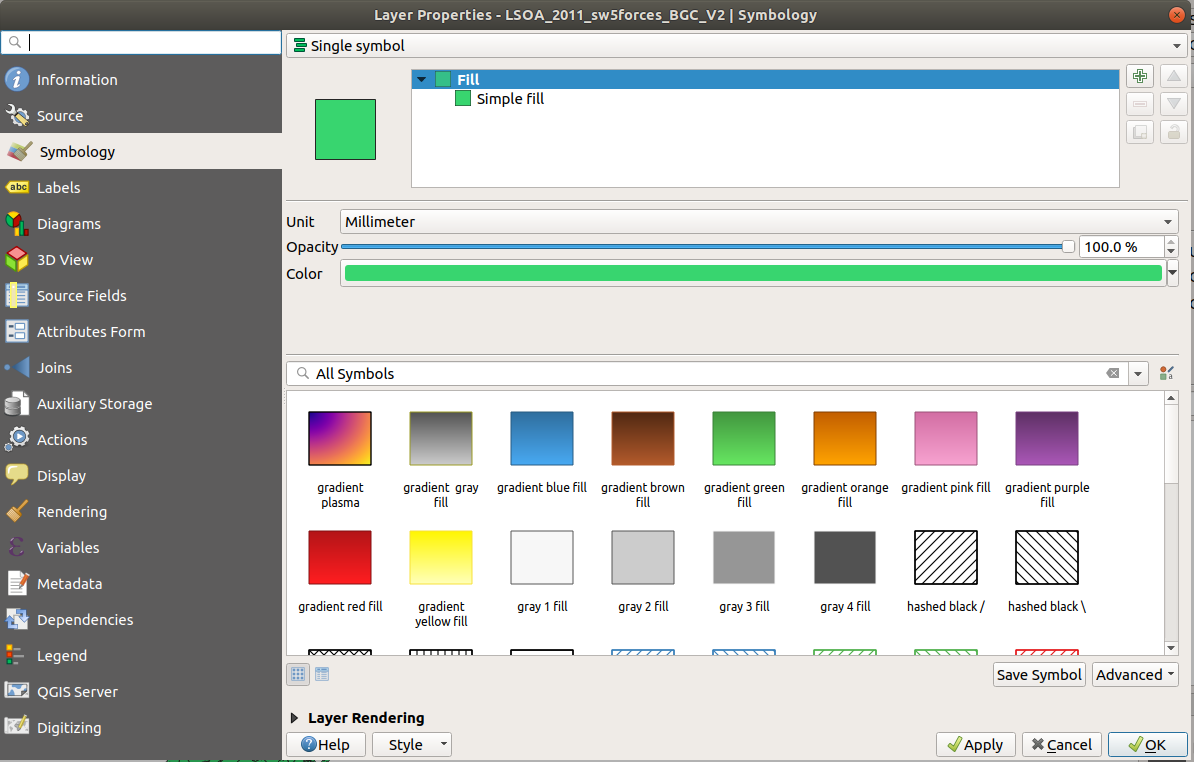
\includegraphics[width=0.8\textwidth]{images/layer_properties_symbology_simple.png}
%	\caption{}
%	\label{ft_fig_firstfig3}
%\end{figure}
%\section{Using the Layer Styling panel}

%Can quickly see how frustrating it is to view the changes while having the \textit{Layer Properties} window in front of the map. We will now move to using the \textit{Layer Styling} panel.

%Enable the \textit{Layer Styling Panel} using the menu (View $\rightarrow$ Panels $\rightarrow$ Layer Styling) or the cick on the icon \begin{tabular}{@{}c@{}}\includegraphics[width=4ex]{images/layers_styling_panel_icon.png}\end{tabular}.\\

%Using the layer styling panel you can simultaneously change the settings and view the map.

Graduated symbology is used to represent continuous fields. We will look at counts of crime per LSOA (the fields we have just joined to the LSOA shapefile).\\

Since these fields all have the same units (count of crime per LSOA) for different categories of crime, when you come to create maps for this type of data, it is often useful at the beginning to consider whether you would like a common colour scale that you will use for all of your fields, or whether you will use a colour scale tailored for each field. This is your choice and will depend on the scale of values in each of your fields.\\
 
The choice of symbology settings (for example number of classes, numerical ranges for each class, the colour scheme) will depend on what you are trying to show. The choices made here make a huge difference to the appearance of your maps.\\

We often ask the data holder to inform us about what to use, so we can represent any important thresholds.\\

Note: the human eye can only detect a difference between a small number (about 8) of monocolours.\\
 
\section{Apply graduated symbology (colours represent numerical ranges)}

Let's quickly put some colour in those shapefile polygons.\\

In the \textit{Layer Styling Panel} ensure the layer to change is selected.\\

Select these settings (leaving the rest as default for now):
\begin{enumerate}[~~~1)]
	\item
Click on \textit{Single symbol} drop down, and choose \textbf{Graduated} (use graduated for continuous data, categorised for classes)
	\item
\textbf{Column}: Choose a column. For example, street\_crime\_Anti-social behaviour
	\item
\textbf{Mode}: Equal Interval
\item
\textbf{Classify}
\end{enumerate}

\null\newpage

\begin{figure}[!h]
	\centering
	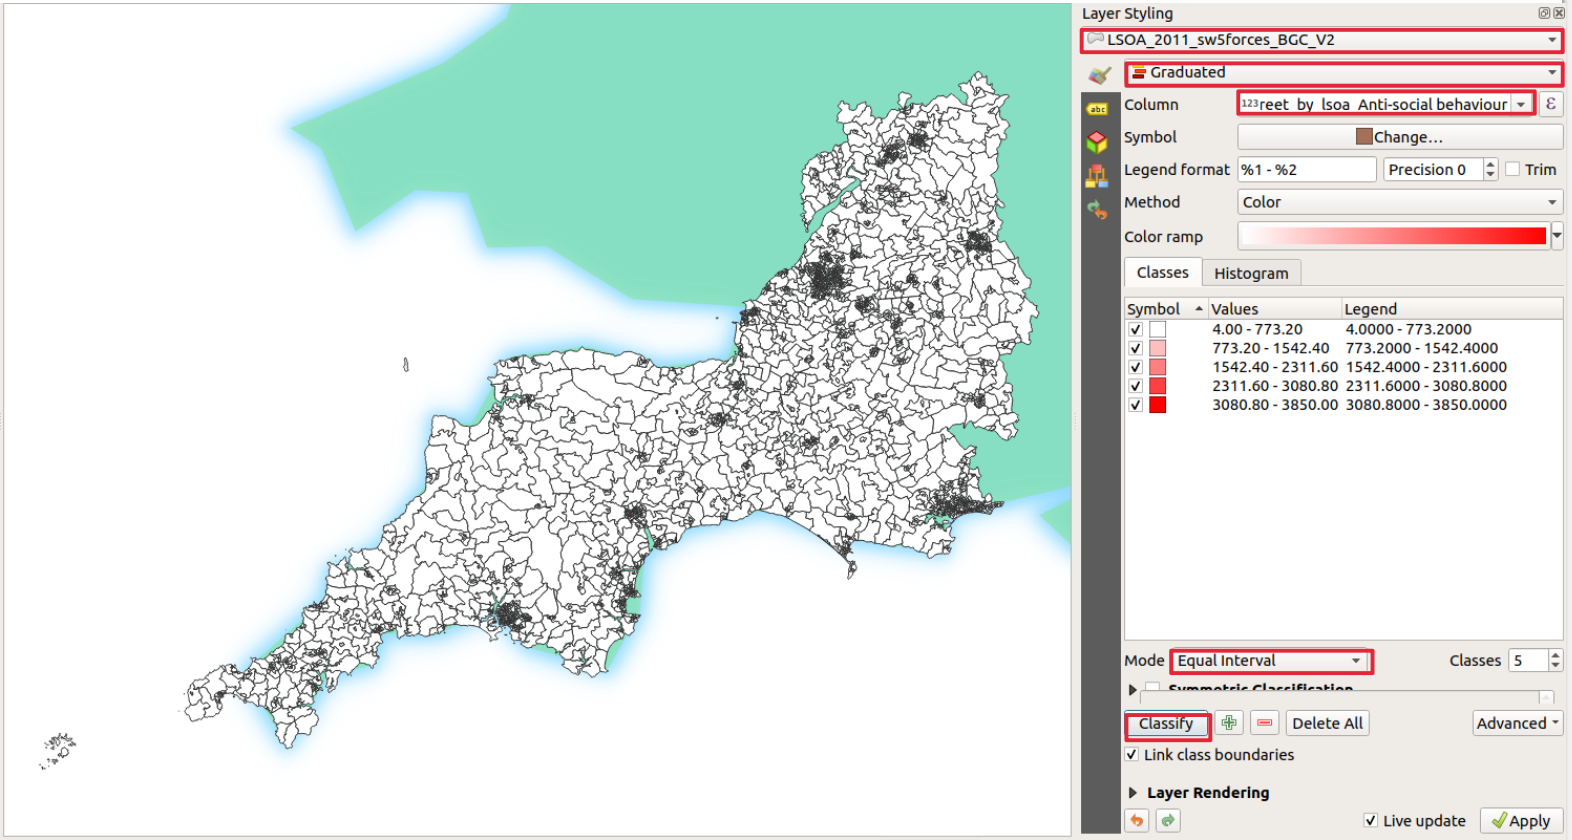
\includegraphics[width=0.8\textwidth]{images/street_crime_graduated1.png}%full_window_layer_styling_panel.png}
	\caption{Graduated symbology to the street crime layer}
	\label{ft_fig_firstfig3}
\end{figure}

\begin{figure}[!h]
	\centering
	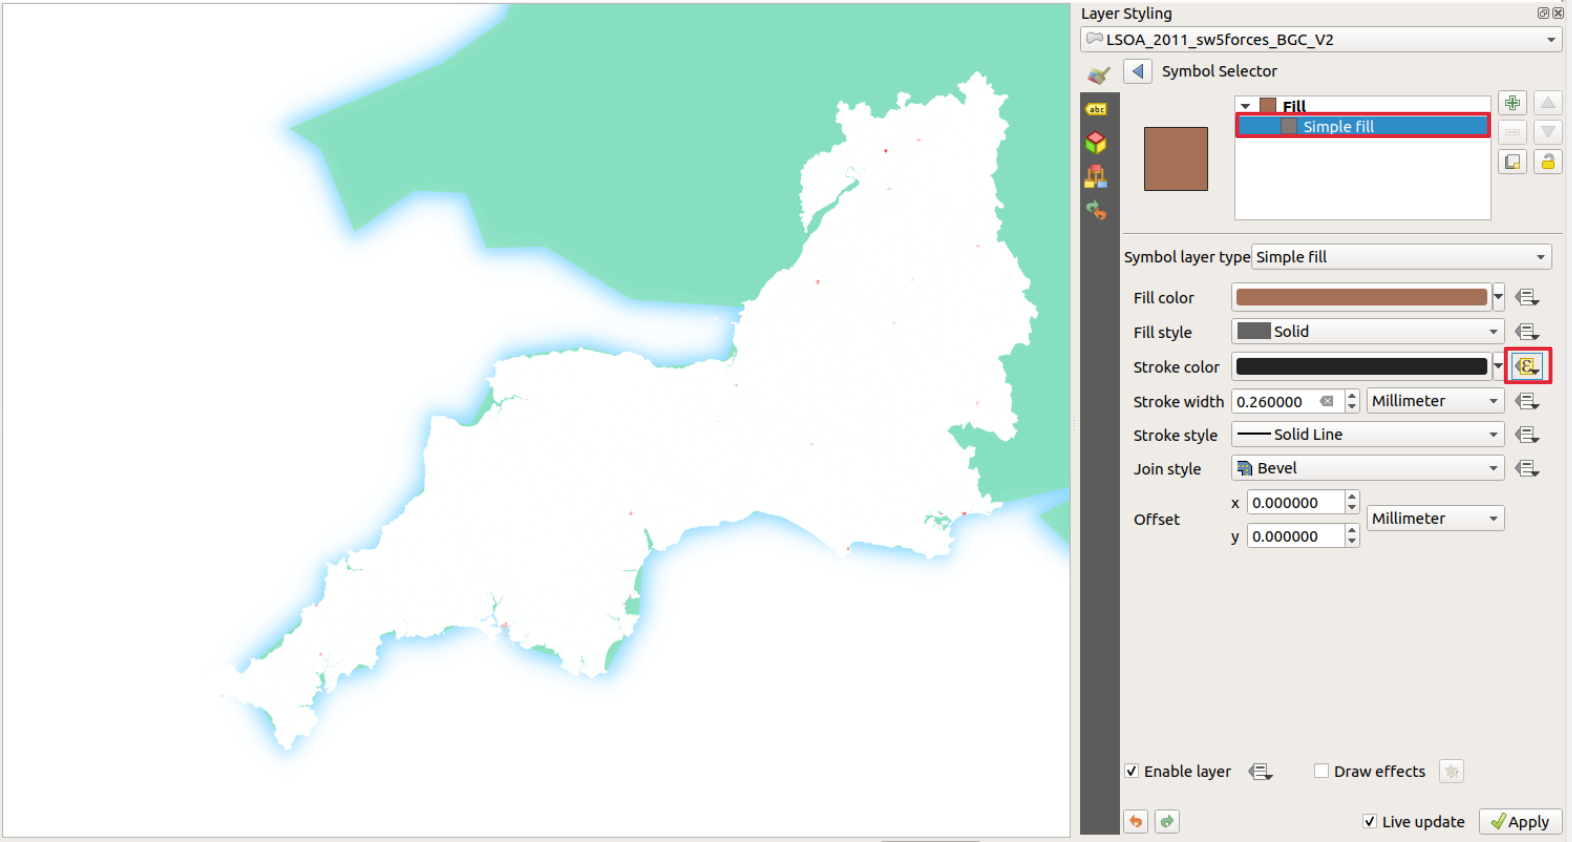
\includegraphics[width=0.8\textwidth]{images/street_crime_stroke_colour.png}%boarders_area_colour3.png}
	\caption{Result of removing the polygon stroke colour}
	\label{ft_fig_firstfig3}
\end{figure}

Each polygon has the corresponding colour to the value in that field. I will explain why it looks like the map has no colour in a bit.\\ 

For the cities with many small polygons it is tricky to see their colour beyond the black boarder. We have a fix for this (see next section).\\

From this, can see we need to increase the width of the UK layers sea colour to maintain a useful basemap.

\null\newpage
\section{Set polygon boarders to automatically have fill colour}

For areas with small polygons (the cities) it is tricky to see the colour beyond the black outline. You can make the polygons outline have the same colour as the fill either by changing each individually, or by using an expression so that it will be done automatically.\\

Make sure nothing is highlighted in the \textit{Layer Styling} pane.\\
Symbol $\rightarrow$ Change\\
Simple fill\\
Stroke color $\rightarrow$ Edit\\
Expression type: $@symbol\_color$\\
OK\\

\begin{figure}[!h]
	\centering
	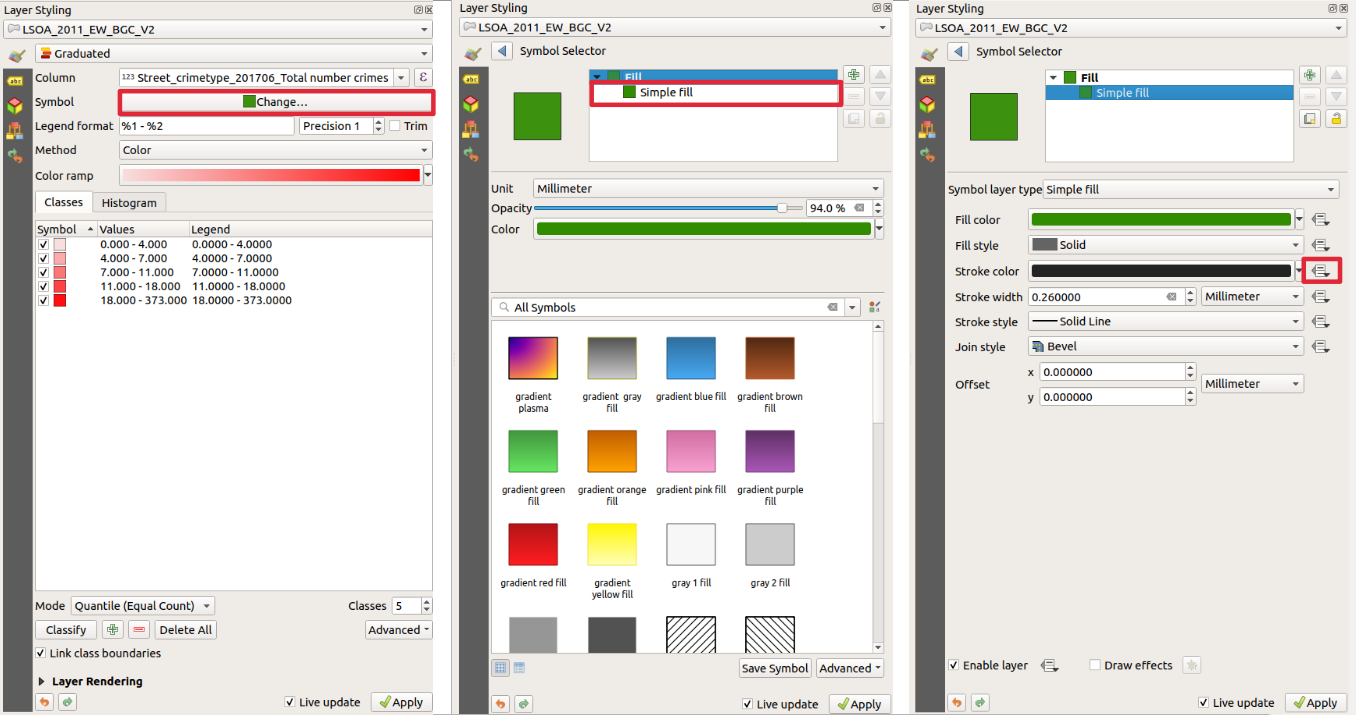
\includegraphics[width=0.9\textwidth]{images/boarders_area_colour1.png}
	\caption{Settings in Layer Styling panel for borders to have same colour as fill (pt 1)}
	\label{ft_fig_firstfig3}
\end{figure}

\begin{figure}[!h]
	\centering
	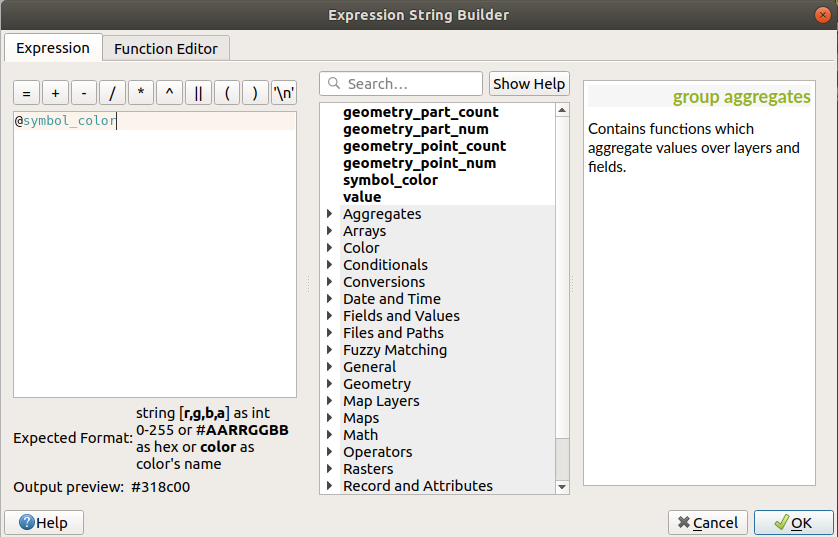
\includegraphics[width=0.5\textwidth]{images/boarders_area_colour2.png}
	\caption{Settings in Layer Styling panel for borders to have same colour as fill (pt 2)}
	\label{ft_fig_firstfig3}
\end{figure}


%\begin{figure}[!h]
%	\centering
%	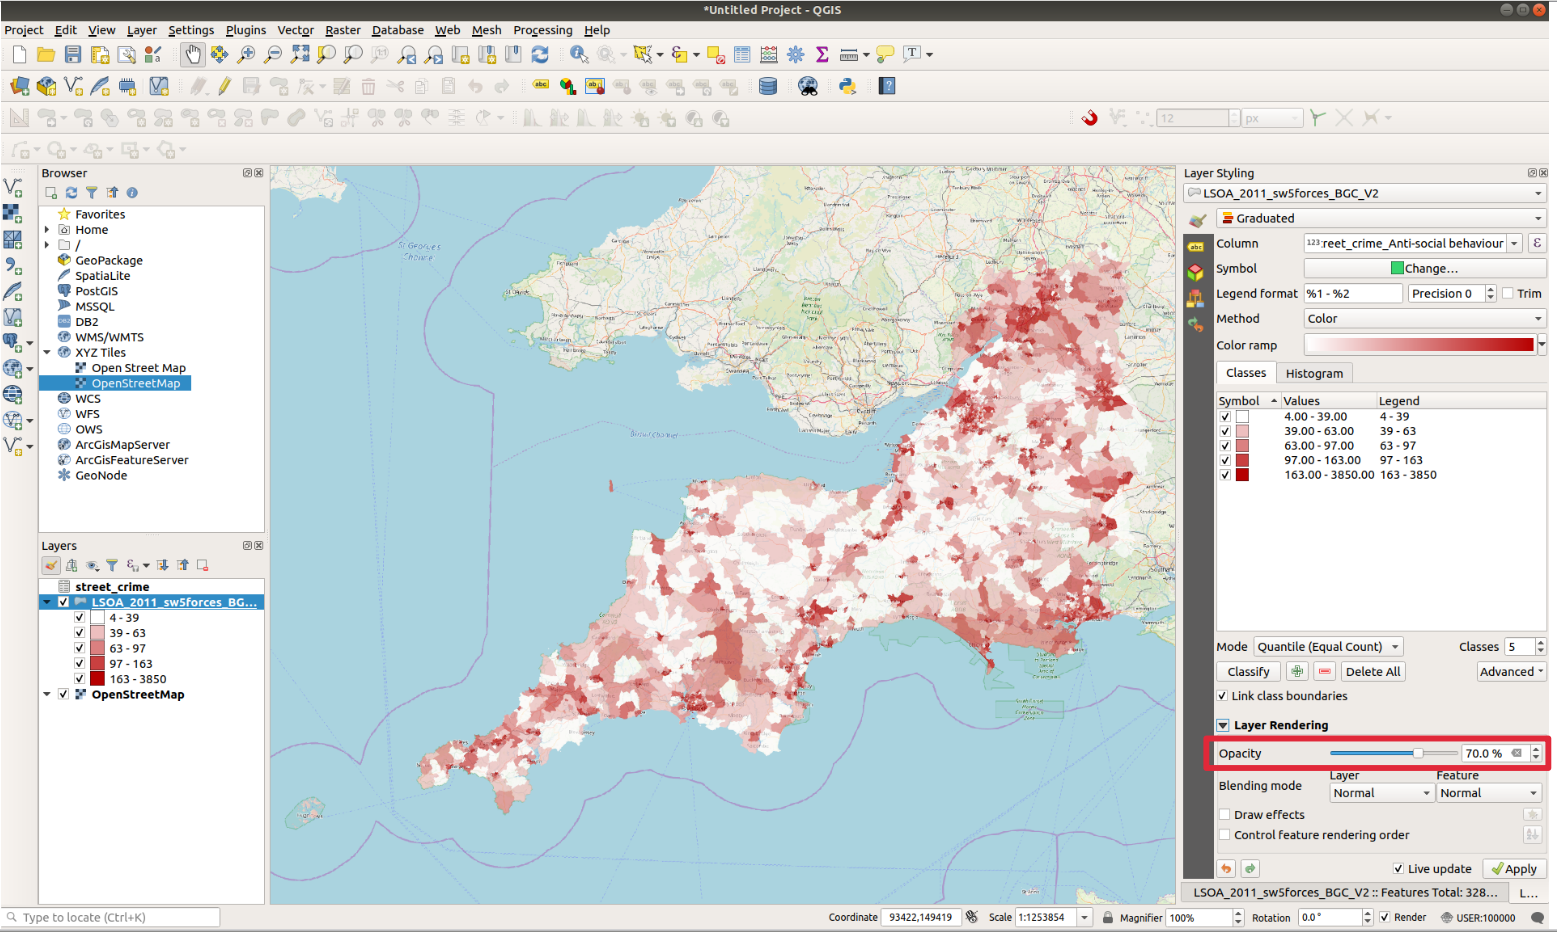
\includegraphics[width=1\textwidth]{images/boarders_area_colour4.png}
%	\caption{}
%	\label{ft_fig_firstfig3}
%\end{figure}

Notice the Edit button is now yellow. Shows that an expression exists there. If want to remove this expression, click on the icon and select clear (you can not delete the expression from the \textit{Expression String Builder} and leave that field blank).\\

If your symbology colour scale includes white, then removing the black outline will lose references to a boundary. This example highlights the importance of using a base map.

\section{Customising and choosing good graduated symbology}

QGIS has many tools to help us select a good colour range. The default one that we have used so far has proven to be not suitable.

\subsection{Use the histogram to inform the number of, \& range for each class band}

Within the \textit{Layer Styling Panel}, view the histogram of the field. Select tab \textit{Histogram} $\rightarrow$ Load Values. If a colour ramp has already been applied to the field, this will be represented in the histogram.\\
Use this to inform the number \& ranges of classes.\\

Note: If you have classes set up, then the histogram will only plot data within that numerical range, and so not necessarily all the data for the chosen column, even when click \textit{Load Values}. If you change the column choice and want to see the full range of data, need to click \textit{classify} first in the \textit{Classes} tab, then view histogram.

\begin{figure}[!h]
	\centering
	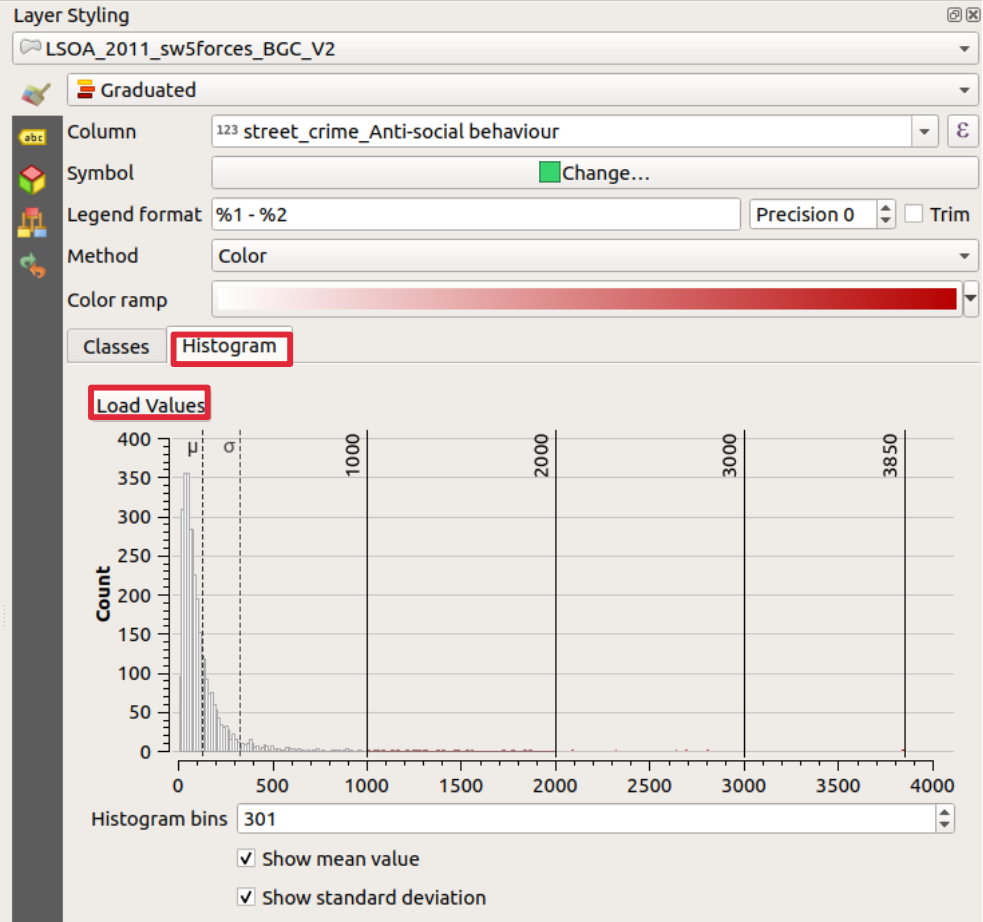
\includegraphics[width=0.7\textwidth]{images/styling_histogram.png}
	\caption{Using histogram to inform graduated symbology}
	\label{ft_fig_firstfig3}
\end{figure}
\null\newpage
\subsection{Use predefined algorithms}

QGIS has 5 modes (predefined methods) to divide your data into discrete classes:\\
Equal Interval, Quantile (equal count), Natural breaks (Jenks), Standard deviation and Pretty breaks. \\

For our case, we had Equal Interval where the full range of the values are divided by the number of classes. For this field there is a large outlier and so most of the polygons fall in the smallest colour band. So for this data, this mode is not suitable.



\begin{figure}[h!] % "[t!]" placement specifier just for this example
	\begin{subfigure}{0.48\textwidth}
		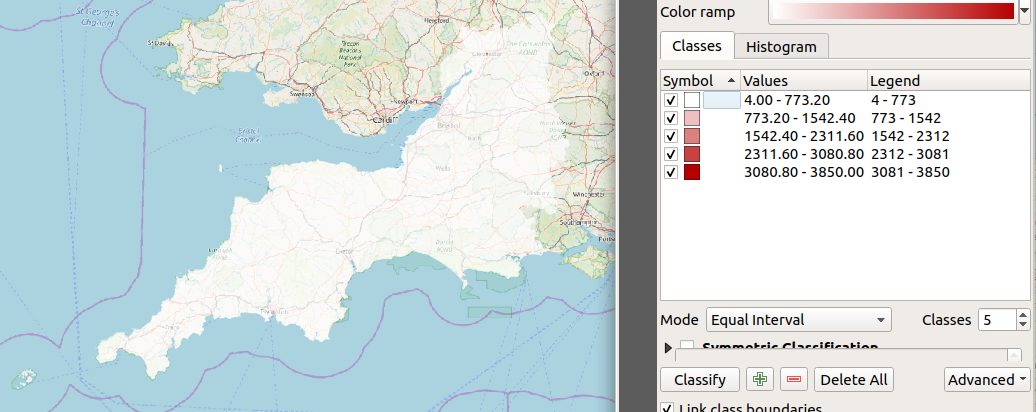
\includegraphics[width=\linewidth]{images/mode_equal_interval.png}
		\caption{Equal interval} \label{Equal interval}
	\end{subfigure}\hspace*{\fill}
	\begin{subfigure}{0.48\textwidth}
		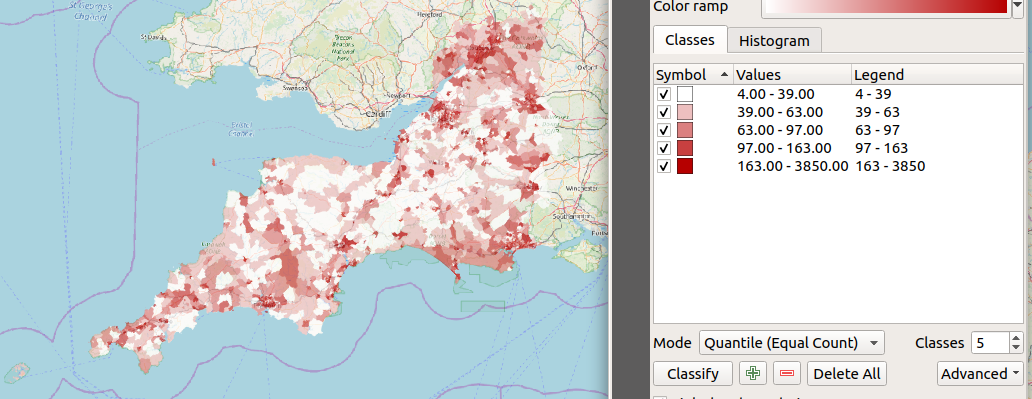
\includegraphics[width=\linewidth]{images/mode_quantile.png}
		\caption{Quantile (Equal count)} \label{Quantile (Equal count)}
	\end{subfigure}
	
	\medskip
	\begin{subfigure}{0.48\textwidth}
		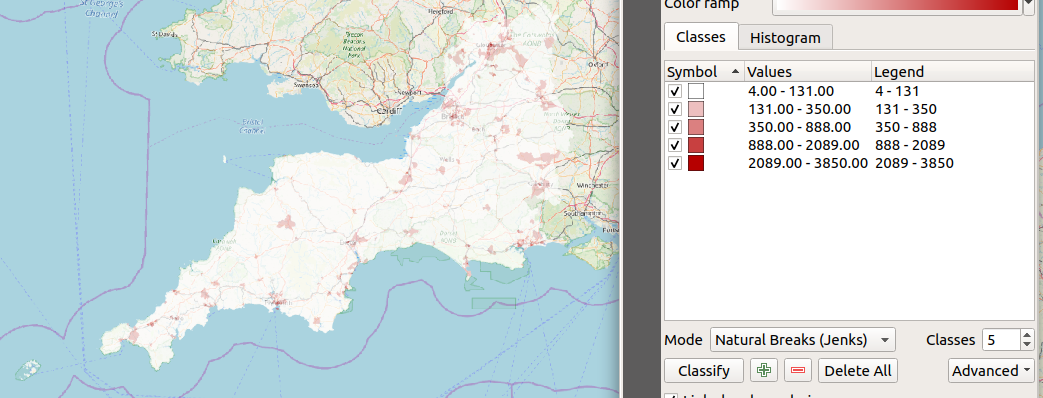
\includegraphics[width=\linewidth]{images/mode_jenks.png}
		\caption{Natural breaks (Jenks)} \label{Natural breaks (Jenks)}
	\end{subfigure}\hspace*{\fill}
	\begin{subfigure}{0.48\textwidth}
		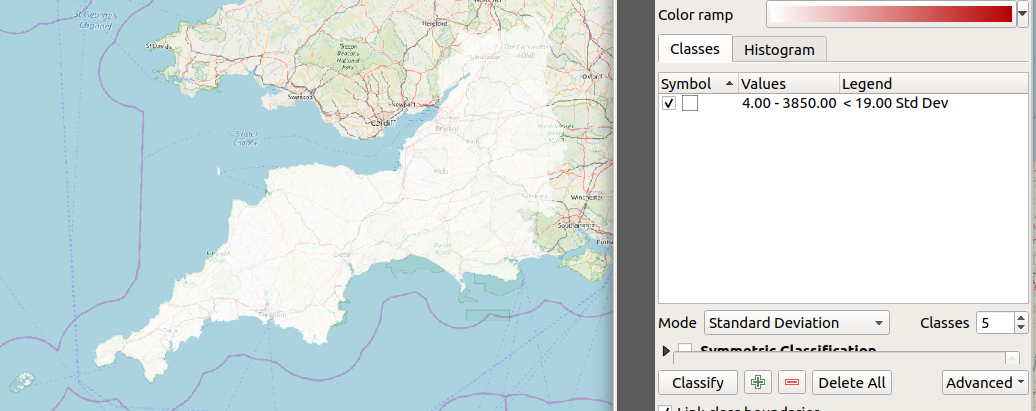
\includegraphics[width=\linewidth]{images/mode_stddev.png}
		\caption{Standard deviation} \label{Standard deviation}
	\end{subfigure}
	
	\medskip
	\begin{subfigure}{0.48\textwidth}
		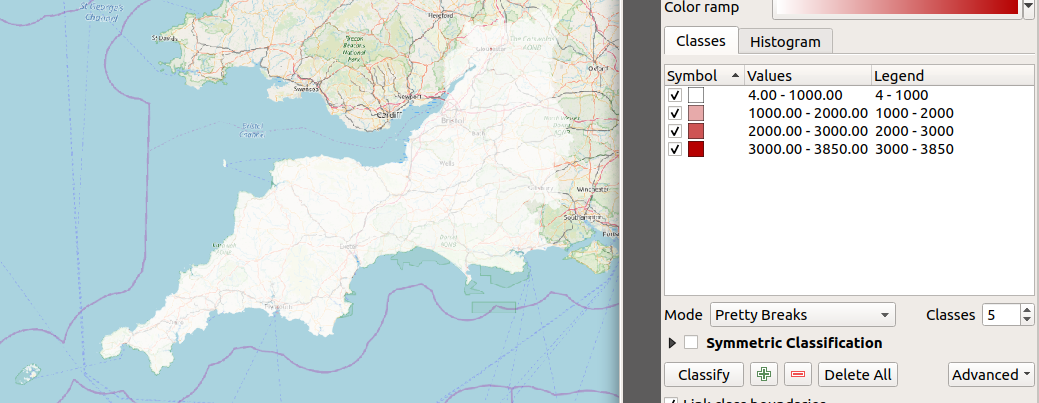
\includegraphics[width=\linewidth]{images/mode_pretty.png}
		\caption{Pretty breaks} \label{Pretty breaks}
	\end{subfigure}\hspace*{\fill}
	
	\caption{The five different algorithms to automatically create graduated bands} \label{fig:1}
\end{figure}

%	A cross-reference to Figure~\ref{fig:1}, and a cross-reference to Subfigure~\ref{fig:e}.

\subsection{Number of classes}
	
Change the number of classes. Your choice 

\subsection{Colour ramp}
	
Can choose one of the predefined colour ramps. Your choice 
	
\subsection{Manually change the symbology}
Instead of using predefined settings, you can also change the symbology of an individual item manually.\\
Within the \textit{Layers Styling Panel}, in the \textit{Classes} tab, double click on the numerical range, or the symbol, to change it.

\subsection{Opacity}
If you have detail in the base map (for example Open Street Map) consider setting this layer's opacity (expand Layers Rendering) to ~60%.
\null\newpage
\begin{figure}[!h]
	\centering
	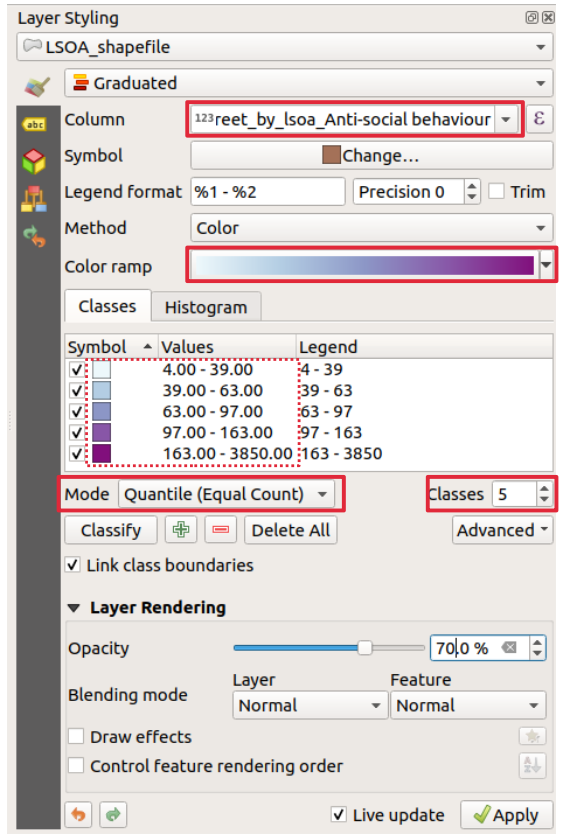
\includegraphics[width=0.4\textwidth]{images/graduated_symbology_options.png}
	\caption{The four red boxes highlight what determines the automatic graduated symbology: column; colour; mode; classes. Double click within the dashed red box to manually change an individual number or colour}
	\label{ft_fig_firstfig3}
\end{figure}
%
%
%\begin{figure}[!h]
%	\centering
%	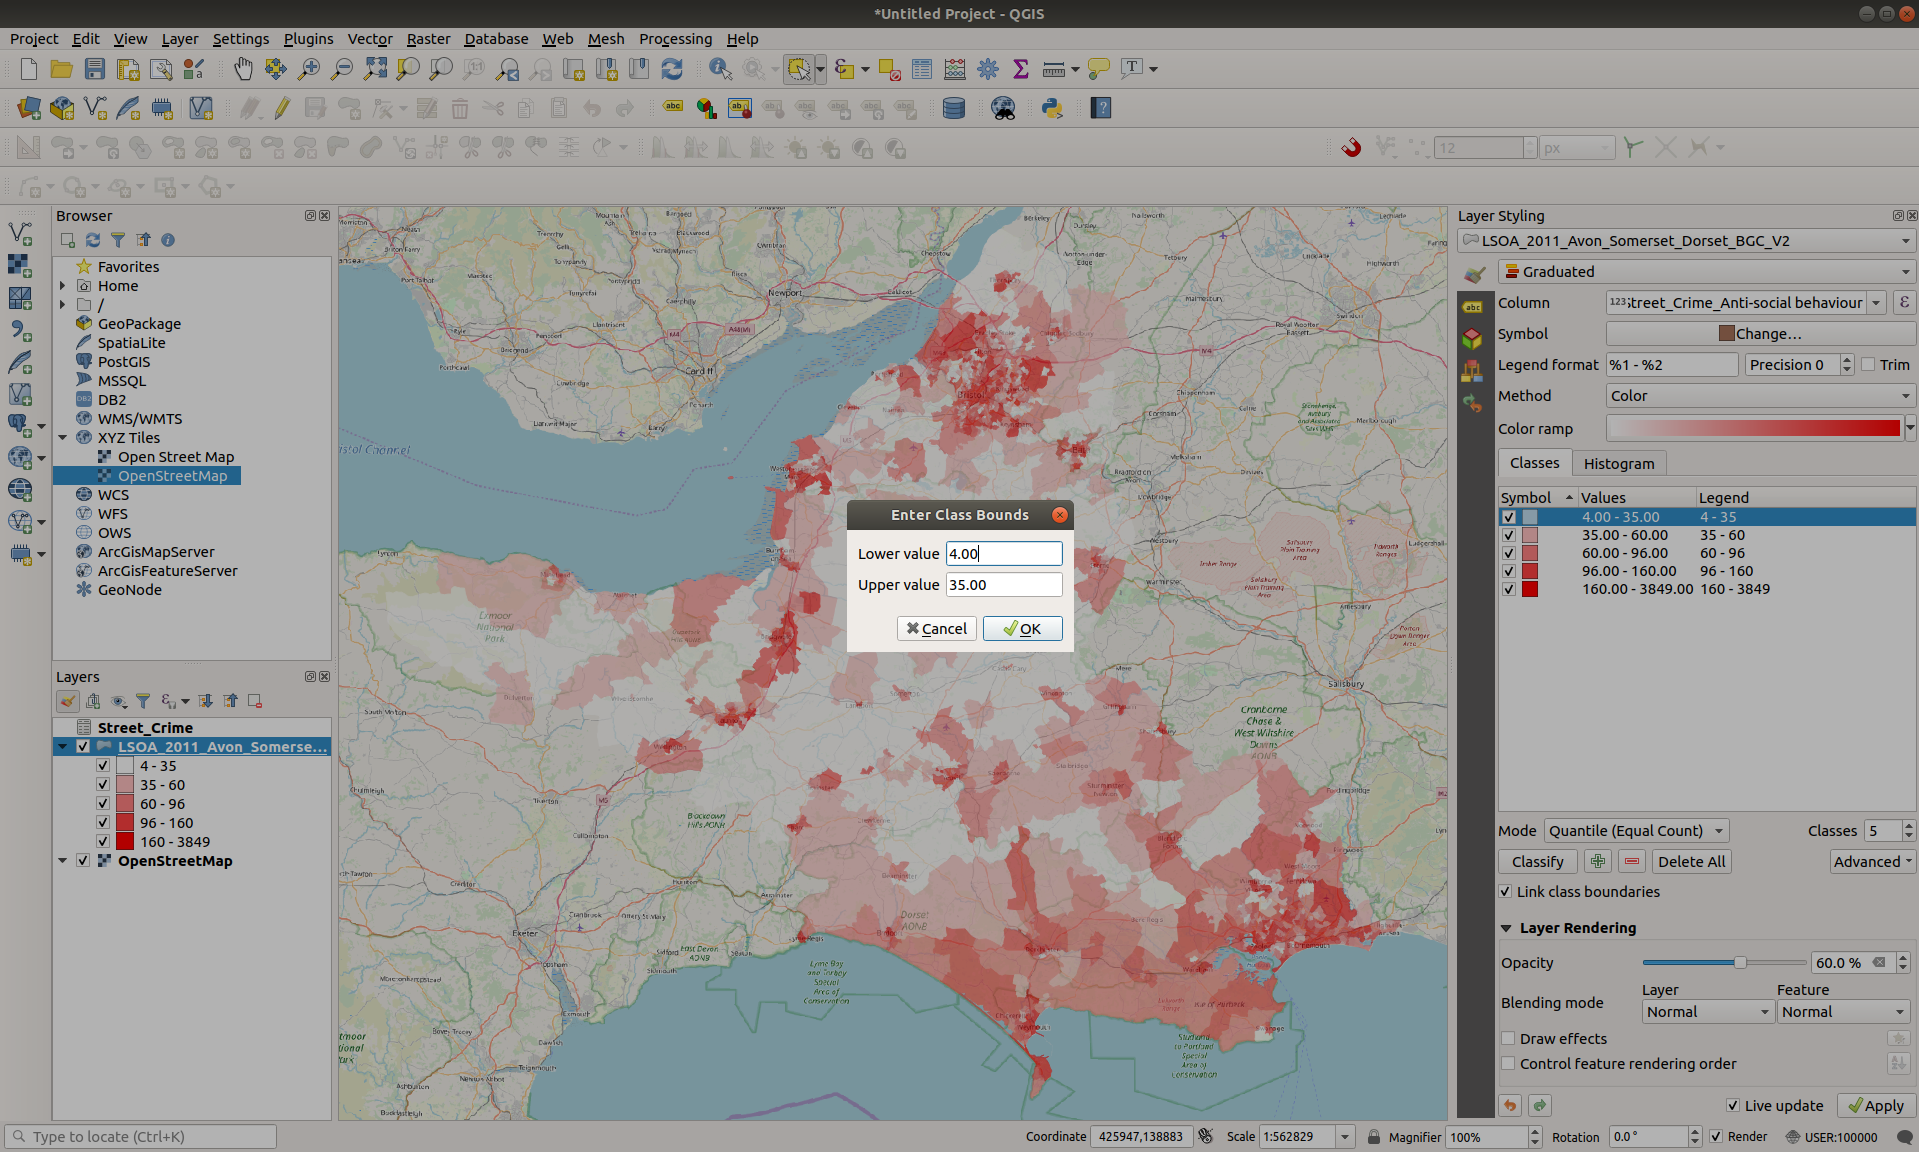
\includegraphics[width=0.6\textwidth]{images/styling_manual.png}
%	\caption{}
%	\label{ft_fig_firstfig3}
%\end{figure}

%\null\newpage

\textbf{TASK}\\
Change the symbology settings to give the most information about the data. There’s no right answer.\\

Note: Two useful buttons at bottom of Layer Styling panel (Undo \& Redo):            
\begin{tabular}{@{}c@{}}
\includegraphics[width=4ex]{images/styling_redo_undo_icon.png}\end{tabular}.\\

%Pan and zoom map so the area of interest takes full screen
%\begin{figure}[!h]
%	\centering
%	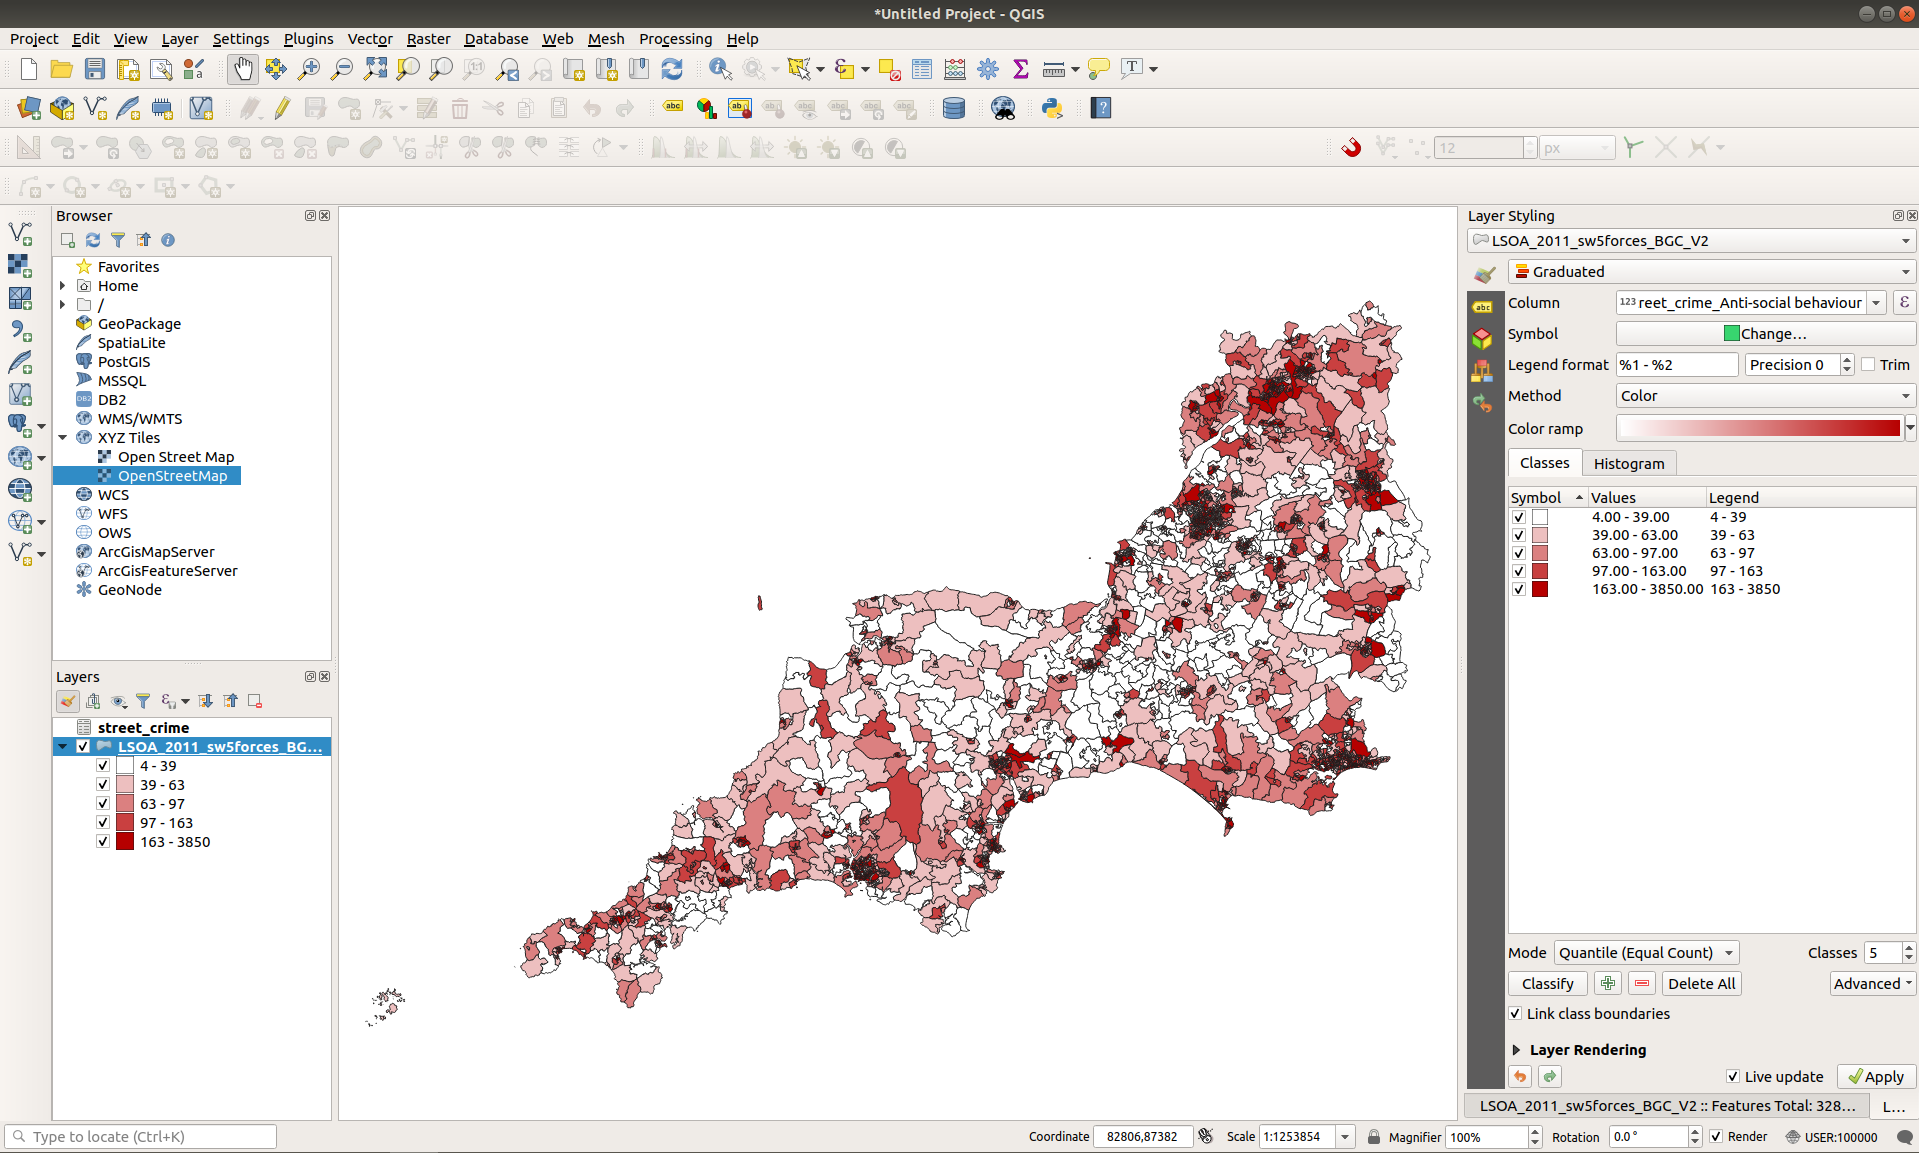
\includegraphics[width=0.85\textwidth]{images/full_window_layer_styling_ASB.png}
%	\caption{}
%	\label{ft_fig_firstfig3}
%\end{figure}

\section{Style the layer with values from another field}

\textit{Unless you made sure the full range of values were included in your symbology, there may be some empty polygons when you change fields and use the same symbology. If want to use the same symbology for multiple columns it’s best to put time into thinking about ranges at the start.}\\

In the \textit{Layer Styling Panel} select a different column: For example, street\_crime\_Bicycle\_theft. Then either:\\

\subsection{Use existing symbology}
Choose your new column, click Apply.\\

\subsection{Update symbology based on new values}
Choose your new column, click classify. The numerical ranges and colours will be overwritten depending on the values in the new column and the symbology settings (mode, classes, color ramp).\\ 


%\begin{figure}[!h]
%	\centering
%	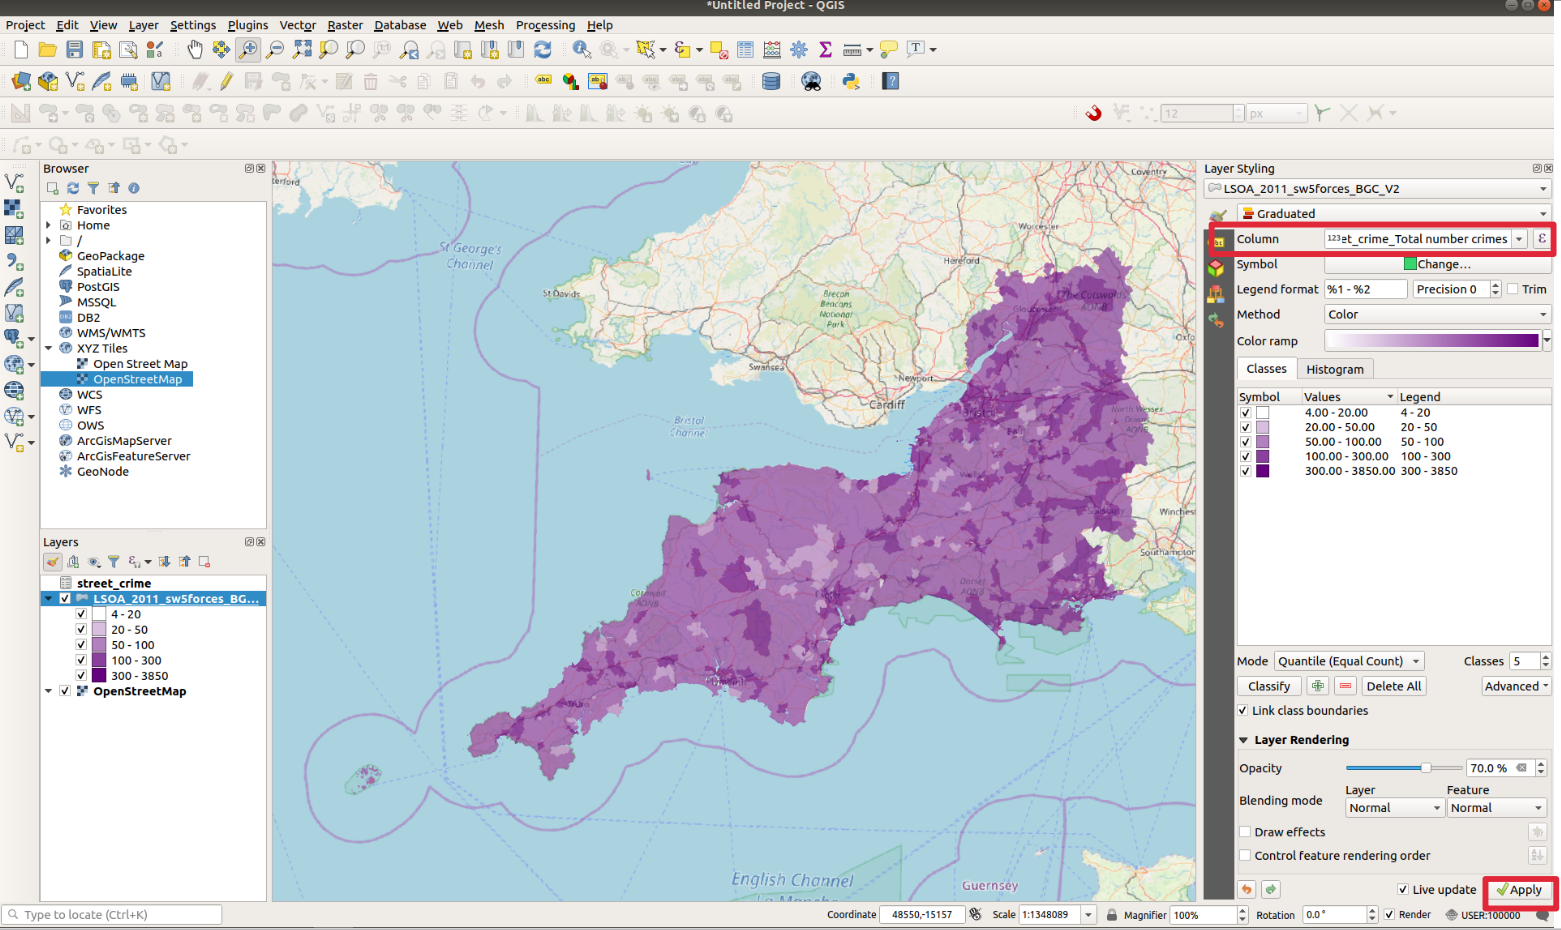
\includegraphics[width=1\textwidth]{images/layer_styling_column_change.png}
%	\caption{}
%	\label{ft_fig_firstfig3}
%\end{figure}

%\begin{figure}[!h]
%	\centering
%	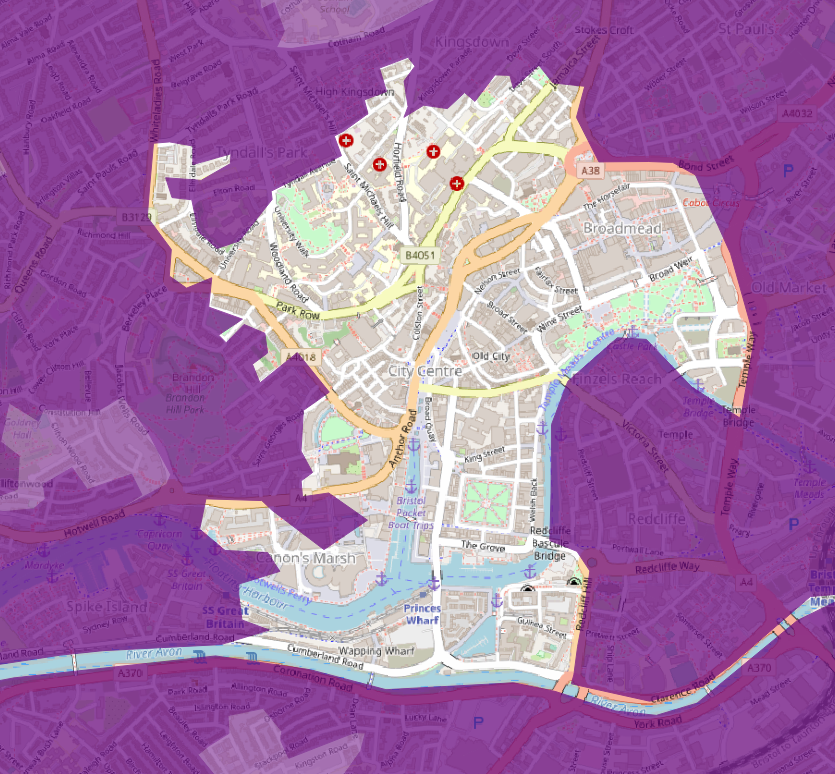
\includegraphics[width=0.4\textwidth]{images/empty_polygon_bristol.png}
%	\caption{}
%	\label{ft_fig_firstfig3}
%\end{figure}

%Set up symbology for this field (as this will have the maximum value)

%\null\newpage
%What could be misleading about this colour choice?

%\begin{figure}[!h]
%	\centering
%	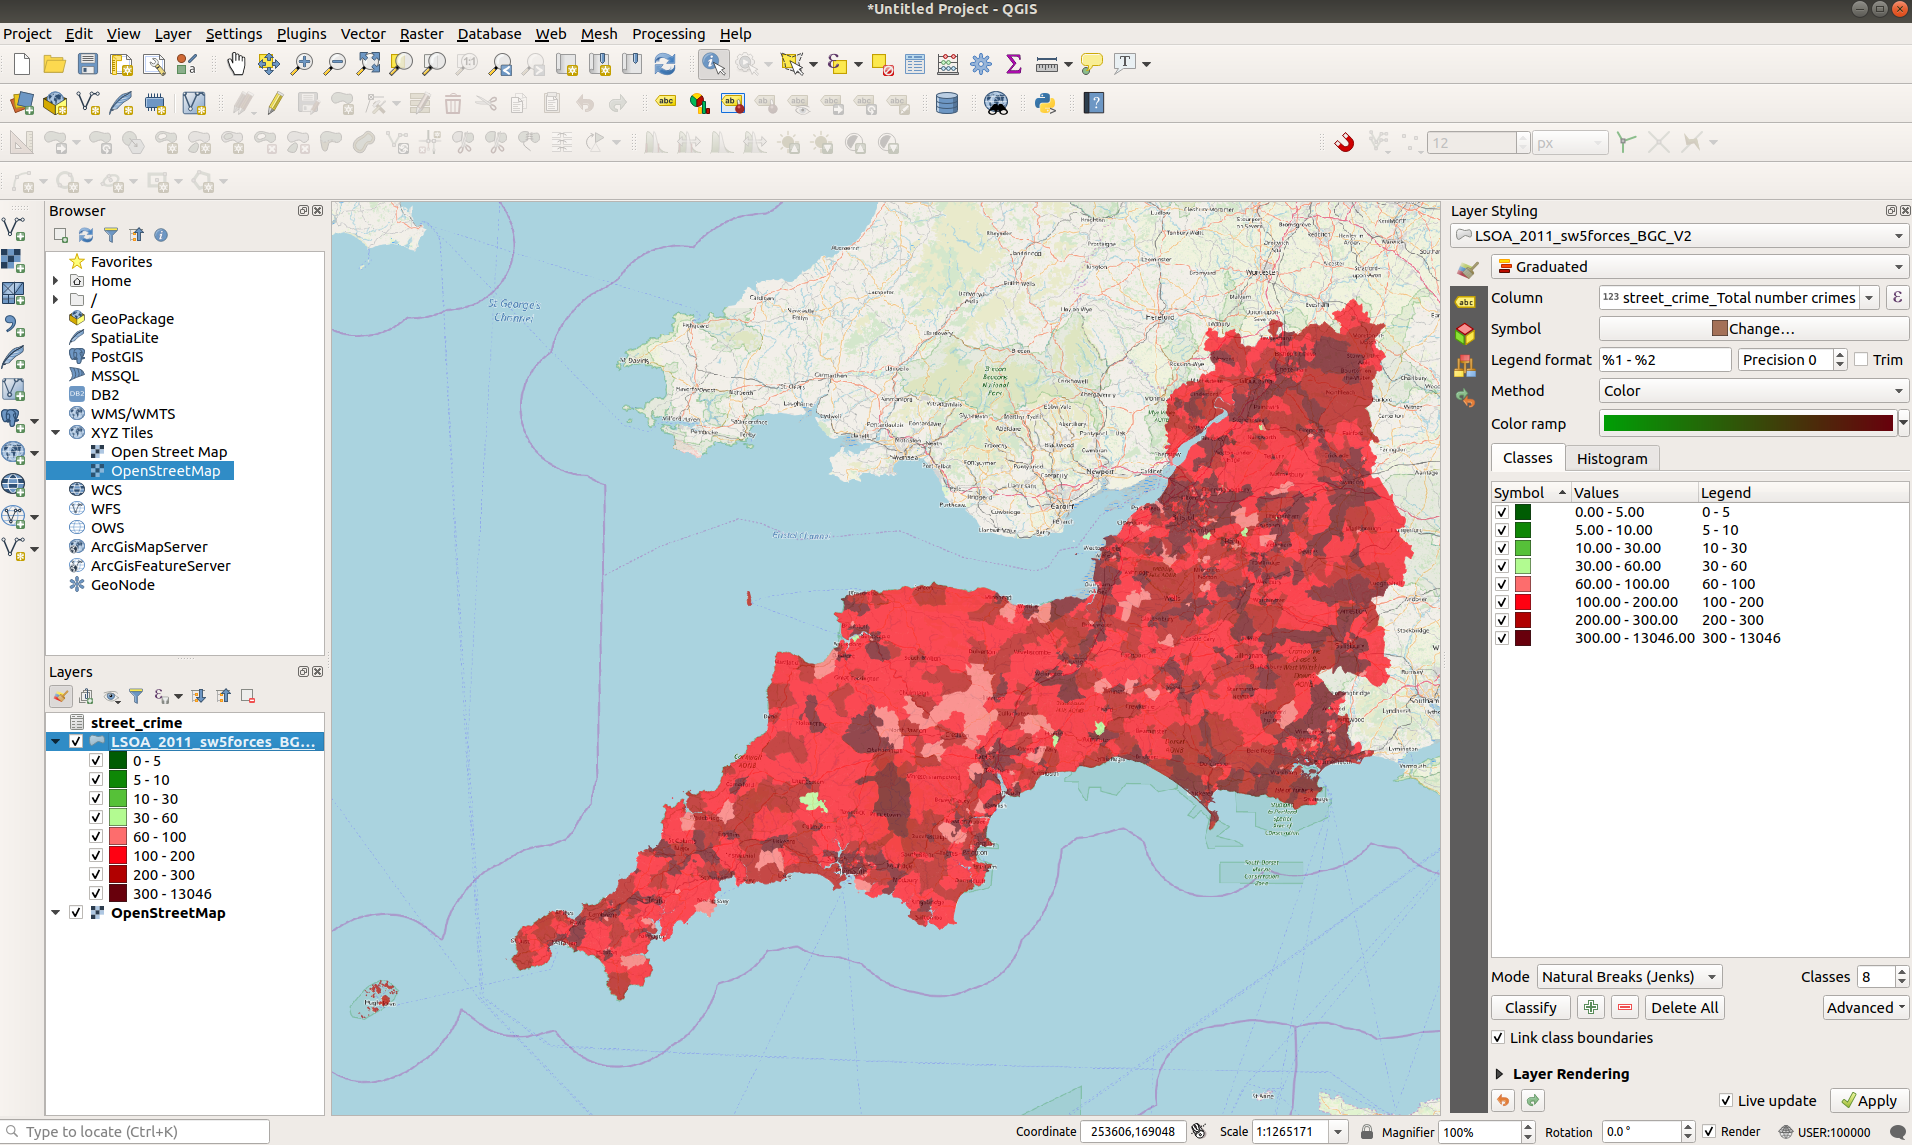
\includegraphics[width=1\textwidth]{images/asb_column_new_style.png}
%	\caption{}
%	\label{ft_fig_firstfig3}
%\end{figure}

\section{Duplicate layer}

Rather than keep changing the column in the same layer, can create duplicates of this layer and have a different column selected for each layer.\\

In the \textit{Layers Panel}, right click on the layer name you want a copy of, select \textit{Duplicate Layer}

\begin{figure}[!h]
	\centering
	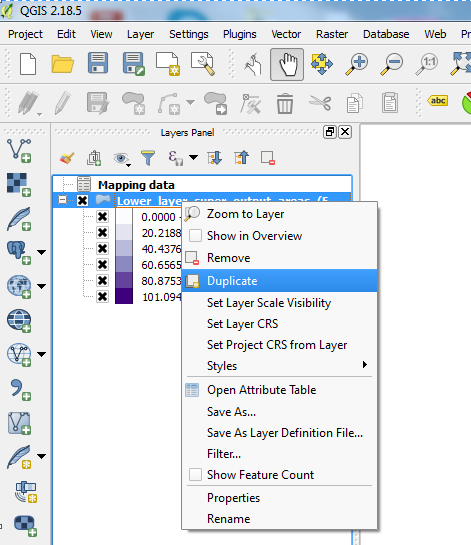
\includegraphics[width=0.4\textwidth]{images/duplicate_layer.png}
	\caption{Create a duplicate layer}
	\label{ft_fig_firstfig3}
\end{figure}

Now we have a duplicate layer, can select the new layer in the \textit{Layer Styling Panel}, and choose a different column, and change the symbology should we require.\\

Click Apply.\\

\section{Copy and paste style}

Lets assume you've noticed an error in the symbology. Make a change to the symbology in the new layer you've just created (e.g. tidy up the legend text).\\
 
Tip: If you want to keep the colours already set, but need an additional class it is best to change the number of classes using the \textbf{+} \& \textbf{-} buttons. If instead I chose to change the number of Classes, this would overwrite the current selection of colours and ranges using the inbuilt algorithms.

\begin{figure}[!h]
	\centering
	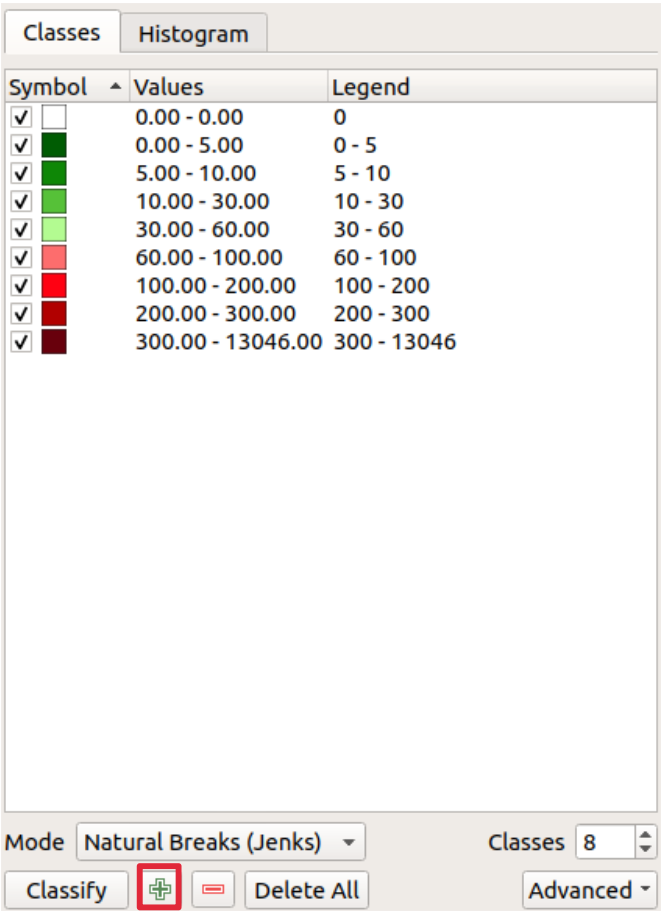
\includegraphics[width=0.3\textwidth]{images/add_class_layer_styling.png}
	\caption{Add or remove a class without overwriting the current symbology}
	\label{ft_fig_firstfig3}
\end{figure}

If you want to use this symbology for the other layer, can copy this symbology and paste it to the other layer:
\begin{enumerate}
	\item 
Right click on the layer with the style you want: Styles $\rightarrow$ Copy style  $\rightarrow$ Symbology
	\item 
Right click on the layer with the style you want to change: Styles $\rightarrow$ Paste Style $\rightarrow$ Symbology 
	\item 
Re-select the column choice
\end{enumerate}

\null\newpage
\section{Save and Load Style}
Once you have a style you like and will likely use in another project, then you can save this style as a file (“.qml”) and load it as a style in a new layer, and in a new QGIS project.\\

There are two mains ways to do this:\\

1. In the \textit{Layers Panel}, Right click on layer name $\rightarrow$ Export $\rightarrow$ Save as QGIS Layer Style File

\begin{figure}[!h]
	\centering
	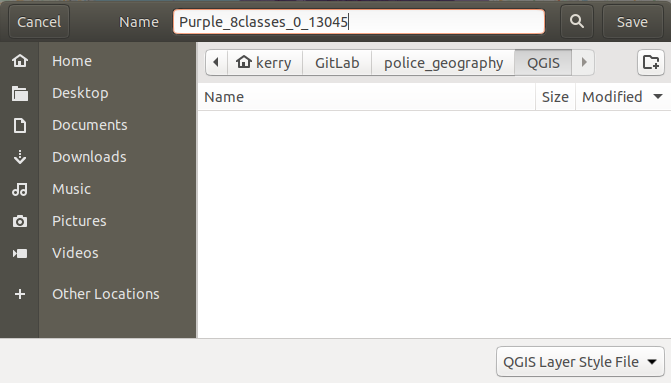
\includegraphics[width=0.5\textwidth]{images/save_as_qgis_layer_style_file.png}
	\caption{Save style from Layers panel}
	\label{ft_fig_firstfig3}
\end{figure}

\null\newpage
2. In the \textit{Layer Properties} window $\rightarrow$ Symbology $\rightarrow$ Style (drop down) $\rightarrow$ Save style.\\

\begin{figure}[!h]
	\centering
	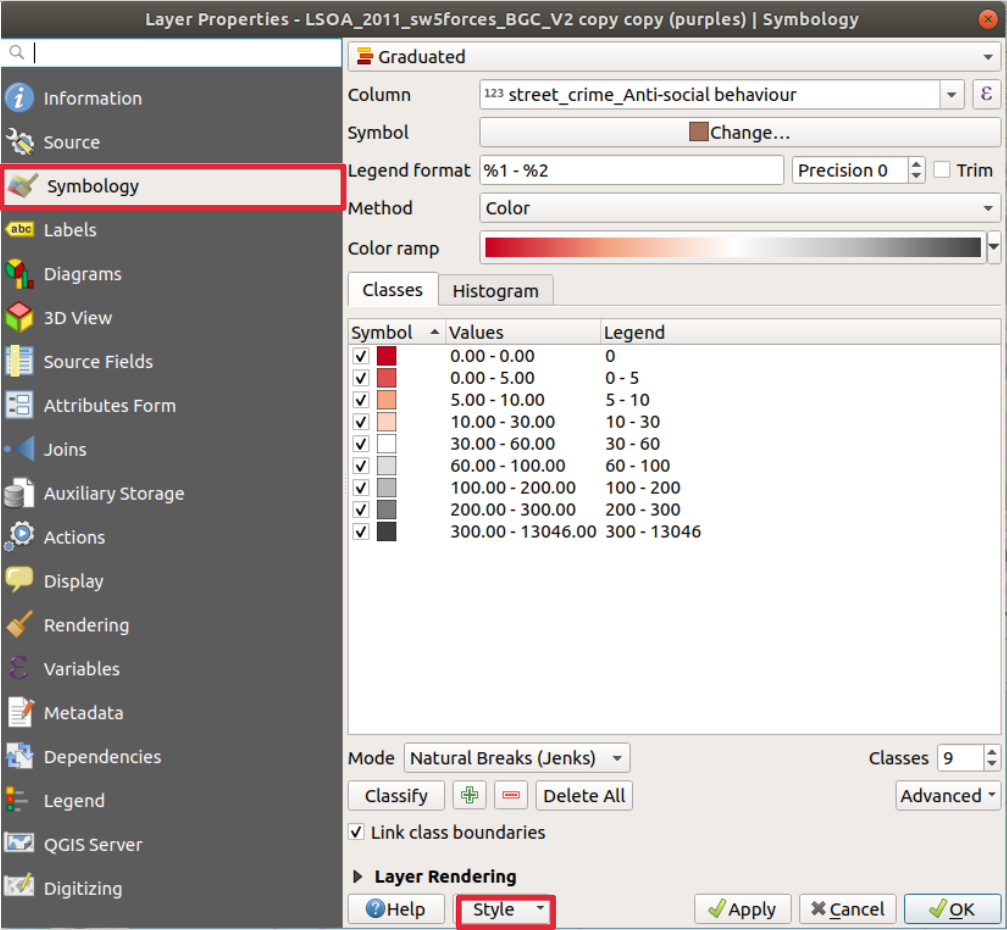
\includegraphics[width=0.6\textwidth]{images/save_style.png}
	\caption{Save style from Layer Properties window}
	\label{ft_fig_firstfig3}
\end{figure}

Load style can be done in the \textit{Layers Styling Panel}.\\

\begin{figure}[!h]
	\centering
	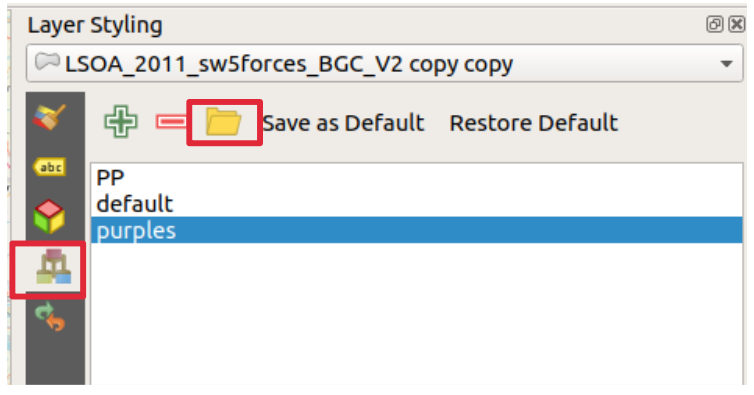
\includegraphics[width=0.4\textwidth]{images/load_style.png}
	\caption{Load style within the Layers Styling panel}
	\label{ft_fig_firstfig3}
\end{figure}

\section{Rename layers}

Now we have multiple layers with very similar names, eg with “(copy)” on the end. Give more useful names to each of these layers. In \textit{Layers Panel} double click on layer name (to open properties window) $\rightarrow$ Source $\rightarrow$ Layer name.\\

Or right click on layer name in \textit{Layers Panel} $\rightarrow$ Rename Layer.
